\section{Baza danych}

\hspace{0.5cm} Baza danych jest to element łączący części systemu stanowiące front-end i back-end. Można ją podzielić na dwie części: przechowującą dane o użytkownikach oraz przechowującą dane o systemie. 

\subsection{Baza danych użytkowników}
\begin{center}
    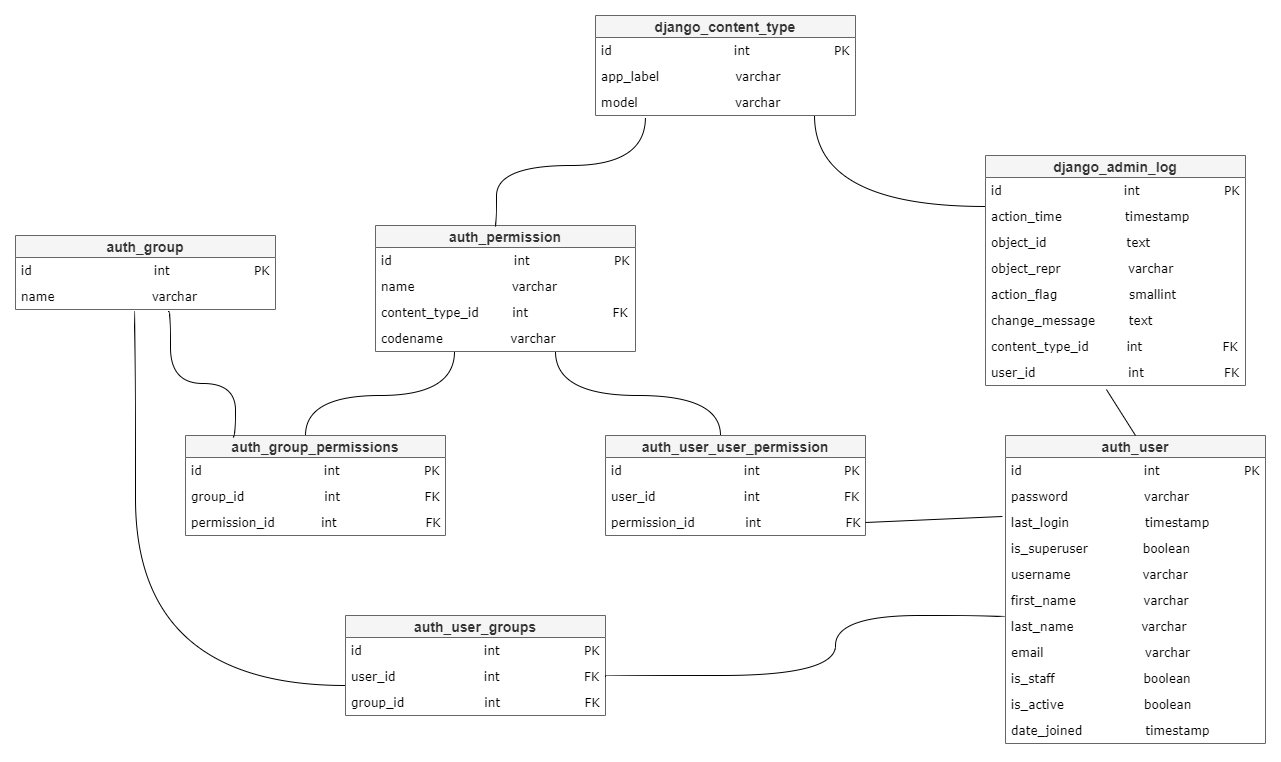
\includegraphics[scale=0.35]{user_database_schema.png}
\end{center}

Baza danych użytkowników została automatycznie stworzona przez framework Django. Umożliwia ona korzystanie z systemu dwóm typom użytkowników: normalnym użytkownikom oraz administratorom. Administrator ma dostęp do wszystkich danych przechowywanych w systemie, może je dowolnie dodawać, usuwać lub edytować. Użytkownik ma dostęp tylko do swoich danych. 

\subsection{Baza danych systemu}
\begin{center}
    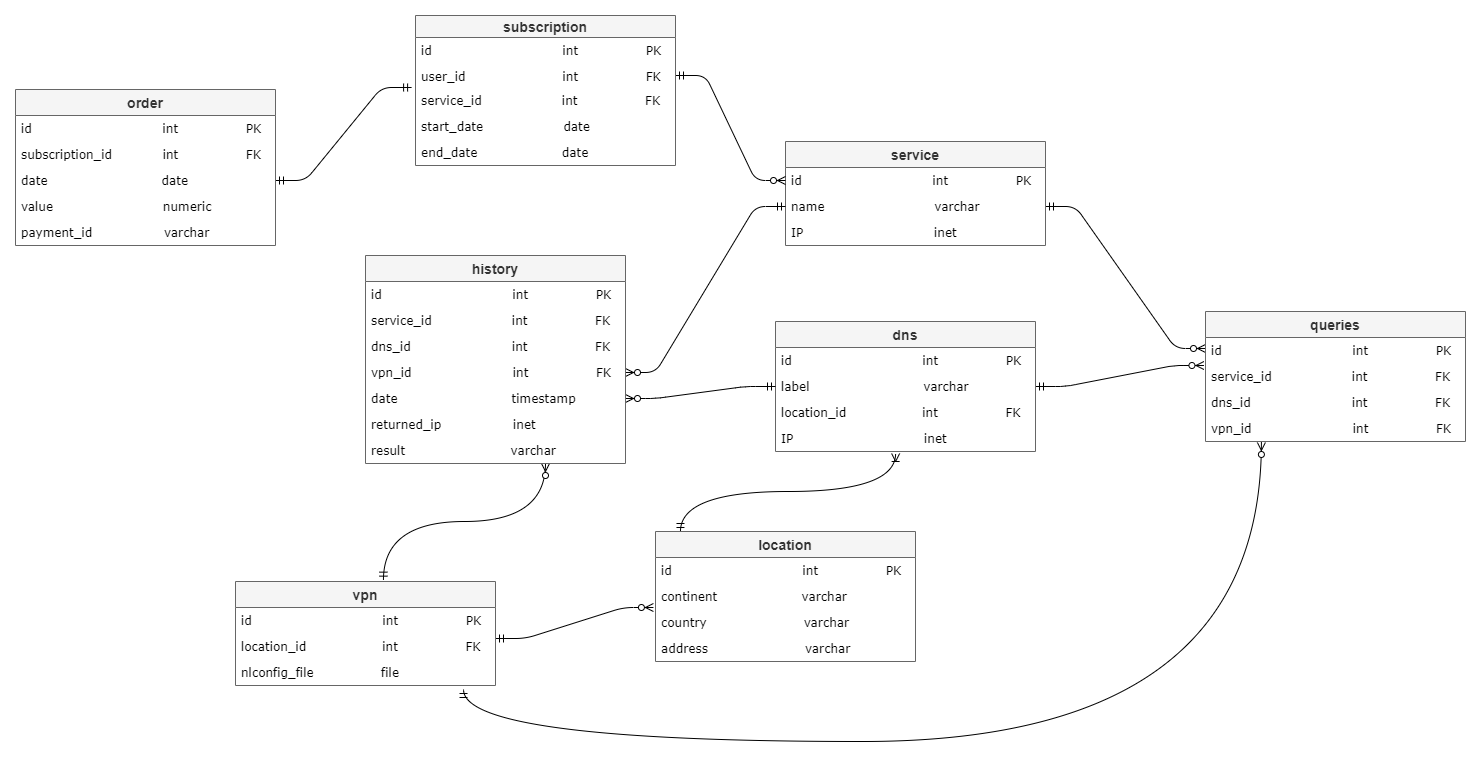
\includegraphics[scale=0.35]{system_database_schema.png}
\end{center}

\noindent
\renewcommand{\arraystretch}{1.7}
\begin{tabular}{p{2cm}p{13cm}}
  \textbf{dns} & tabela przechowująca znane systemowi serwery dns, \\
  \textbf{history} & tabela zawierająca historię odpytywania serwerów dns o poszczególne serwisy, z uwzględnioną datą i rezultatem,\\
  \textbf{location} & lokalizacja, miejsce gdzie znajduje się serwer dns, lub gdzie prowadzi vpn, \\
  \textbf{order} & tabela zawierająca szczegóły zamówienia: datę zatwierdzenia, wartość oraz numer płatności, \\
  \textbf{queries} & tabela łącznikowa, łącząca serwis z serwerami dns które należy sprawdzać oraz lokalizacjami, z których należy sprawdzać poprawność zapytań, \\
  \textbf{service} & tabela przechowująca dane o serwisach klientów, które należy sprawdzać, \\
  \textbf{subscription} & tabela zawierająca informację o subskrypcji, w tym datę rozpoczęcia i wygaśnieęcia, \\
  \textbf{vpn} & tabela zawierająca pliki konfiguracyjne vpn'ów,
\end{tabular}
